\documentclass[12pt]{exam}
\usepackage{amsthm}
\usepackage{libertine}
\usepackage[utf8]{inputenc}
\usepackage[margin=1in]{geometry}
\usepackage{amsmath,amssymb}
\usepackage{multicol}
\usepackage[shortlabels]{enumitem}
\usepackage{siunitx}
\usepackage{cancel}
\usepackage{graphicx}
\usepackage{pgfplots}
\usepackage{listings}
\usepackage{tikz}


\pgfplotsset{width=10cm,compat=1.9}
\usepgfplotslibrary{external}
\tikzexternalize

\newcommand{\class}{Física Moderna - Complementaria} % This is the name of the course 
\newcommand{\examnum}{Taller 3} % This is the name of the assignment
\newcommand{\examdate}{03/03/2023} % This is the due date
\newcommand{\timelimit}{}





\begin{document}
\pagestyle{plain}
\thispagestyle{empty}

\noindent
\begin{tabular*}{\textwidth}{l @{\extracolsep{\fill}} r @{\extracolsep{6pt}} l}
	\textbf{\class} & \textbf{Name:} & \textit{Sergio Montoya Ramirez}\\ %Your name here instead, obviously 
\textbf{\examnum} &&\\
\textbf{\examdate} &&\\
\end{tabular*}\\
\rule[2ex]{\textwidth}{2pt}
% ---

\begin{enumerate} %You can make lists!
	\item A partir de la ley de radiación de Plank:
		\begin{align}
			I(\lambda, T) = \frac{2\pi c^2h}{\lambda^5}\frac{1}{e^{\frac{\beta hc}{\lambda}}-1}
		\end{align}
		\begin{itemize}
			\item Demostrar la ley de Wien

				Para esto, lo que nos interesa es encontrar la longitud de onda que maximiza la Intensidad. Sin embargo, lo primero que podemos hacer es obligar a que T tome un valor, en particular haremos que $T = T$. entonces esto nos deja con:
				\begin{align*}
					I(\lambda) = \frac{2\pi c^2h}{\lambda^5}\frac{1}{e^{\frac{\beta hc}{\lambda}}-1}
				\end{align*}
				Donde la unica variable es $\lambda$ con esto ya en mente podemos derivar, en una sola variable, pues lo que nos interesa es un punto maximo. Por lo tanto ahora le sacamos su derivada lo cual seria.
				\begin{align*}
					I'(\lambda) = -\frac{2\pi c^2 h}{\lambda^6}\frac{1}{e^{\frac{\beta hc}{\lambda}}-1}+\frac{2\pi c^2h}{\lambda^5}\frac{\beta hc e^{\frac{\beta hc}{\lambda}}}{\lambda^2(e^{\frac{\beta hc}{\lambda}}-1)^2}
				\end{align*}
				Ahora con esto podemos encontrar el maximo haciendo que la derivada sea 0 lo cual nos deja con la expresión
				\begin{align*}
					\frac{2\pi c^2h}{\lambda^6}\frac{1}{e^{\frac{\beta hc}{\lambda}}-1}=\frac{2\pi c^2h}{\lambda^5}\frac{\beta hc e^{\frac{\beta hc}{\lambda}}}{\lambda^2(e^{\frac{\beta hc}{\lambda}}-1)^2}
				\end{align*}
		Con esto entonces podemos cancelar varios valores y nos queda
		\begin{align*}
			\frac{\cancel{2\pi c^2h}}{\cancel{\lambda^6}}\frac{1}{\cancel{e^{\frac{\beta hc}{\lambda}}-1}}=\frac{\cancel{2\pi c^2h}}{\cancel{\lambda^5}}\frac{\beta hc e^{\frac{\beta hc}{\lambda}}}{\cancel{\lambda^2}\cancel{(e^{\frac{\beta hc}{\lambda}}-1)^2}}
		\end{align*}
		Lo que al final se expresa como
		\begin{align*}
			\lambda = \frac{\beta hce^{\frac{\beta hc}{\lambda}}}{e^{\frac{\beta hc}{\lambda}}-1}
		\end{align*}
		Sin embargo, esto es ligeramente problematico dado que la anterior es una función trascendental que para solucionar tendriamos que abrir en series de Fourier. Aun asi, tenemos otra aproximación quizas un poco mas simplista que seria convertir $\beta hc$ en una constante de valor arbitrario y encontrar valores numericos en los cuales estos sean iguales. Con esta manera entonces nos queda
				\begin{align*}
					\lambda = \frac{X e^{\frac{x}{\lambda}}}{e^{\frac{x}{\lambda}}-1}
				\end{align*}
				
				Que se puede ver graficamente en la imagen \ref{fig:Imagen_Absurda_2}
				\begin{figure}[ht]
					\centering
					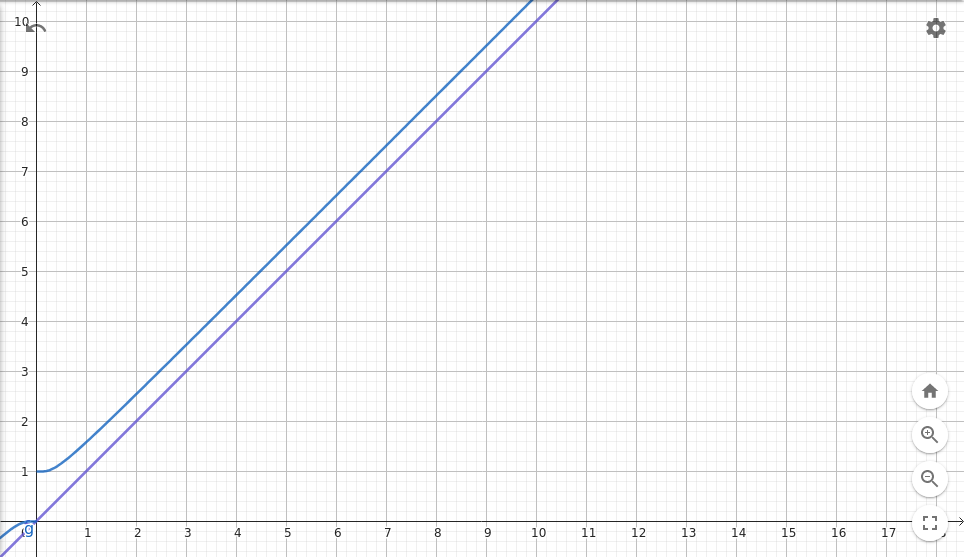
\includegraphics[scale=0.4]{Imagen_Absurda_2.png}
					\caption{Imagen de la ecuación encontrada justamente antes, en ella x toma un valor absurdo de 1. pero esto permite mostrar la correlación entre ambos valores.}
					\label{fig:Imagen_Absurda_2}
				\end{figure}
			\item Demuestre la ley de Rayleight-Jeans
				
				Sabemos que la ley de Rayleight-Jeans funciona muy bien con $\lambda$ muy grande. Por lo tanto, nos podria interesar investigar los casos en donde estos se hagan iguales. En particular podemos partir
				\begin{align*}
					&\frac{2\pi cK_B T}{\lambda^4} = \frac{2\pi c^2h}{\lambda^5}\frac{1}{e^{\frac{\beta hc}{\lambda}}-1}\\
					&\frac{\cancel{2\pi c}K_B T}{\cancel{\lambda^4}} = \frac{\cancel{2\pi} \cancel{c^2}h}{\cancel{\lambda^5}}\frac{1}{e^{\frac{\beta hc}{\lambda}}-1}\\
					&\frac{\lambda}{\beta hc} = \frac{1}{e^{\frac{\beta hc}{\lambda}}-1}
				\end{align*}
				Y como ya habiamos dicho previamente nos encontramos que esta es una ecuación trascendental y por lo tanto respondamos de manera grafica haciendo que $\beta hc$ sea una constante c y graficando nos quedaria mas o menos como en la figura \ref{fig:Imagen_Absurda}
				\begin{figure}[h!]
					\centering
					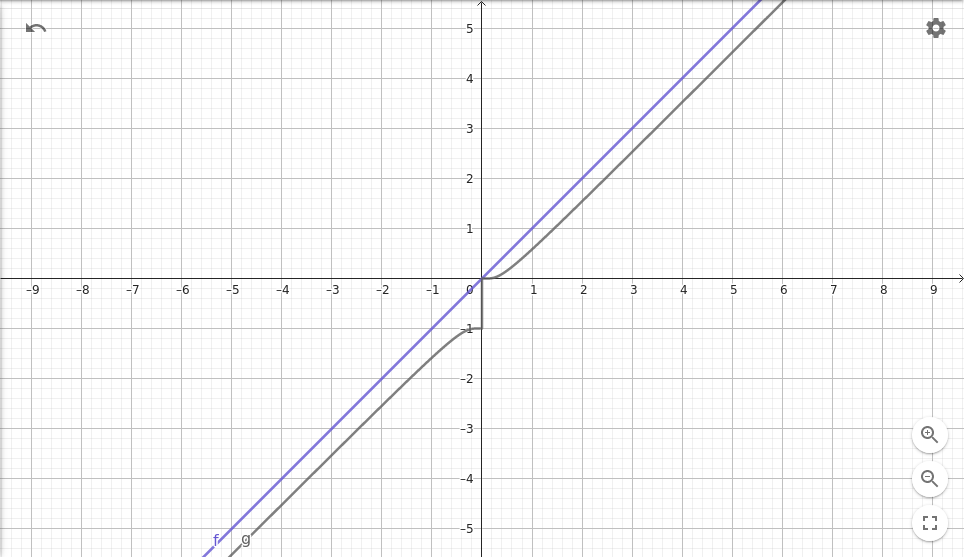
\includegraphics[scale=0.4]{Imagen_Absurda.png}
					\caption{Grafica de la igualdad hayada previamente, esta se hizo con un valor para $\beta hc$ absurdo (el valor utilizado fue 1) pero tenia el objetivo de mostrar mas o menos la correlación entre ambos.}
					\label{fig:Imagen_Absurda}
				\end{figure}

				Ademas, para mostrar la gran correlación que hay los valores con $\lambda = 50$ es 50 y 49.50 respectivamente lo que muestra lo similares que resultan estos valores.

			\item Demuestre la ley de Stefan Boltzman

				Para demostra esta ley debemos integrar con respecto a la longitud de onda e igualar con respecto a $\epsilon\sigma T^4$ lo que nos daria
				\begin{align*}
					&\int_0^\infty I(\lambda) d\lambda = \int_0^\infty \frac{2\pi c^2h}{\lambda^5}\frac{1}{e^{\frac{\beta hc}{\lambda}}-1}d\lambda
				\end{align*}
				Esta integral resulta mas sencilla si hacemos una sustitución (ademas de sacar las constantes) con el valor al que esta elevado $e$ pues asi nos quedaria
				\begin{align*}
					&x = \frac{\beta hc}{\lambda}\\
					&dx = -\frac{\beta hc}{\lambda^2}d\lambda\\
					&2\pi c^2h \int \frac{-\frac{\lambda^2}{\beta hc}dx}{\lambda^5(e^x -1)}\\
					&\frac{2 \pi c^2h}{\beta hc}\int -\frac{1}{\lambda^3(e^x-1)}dx\\
					&\lambda = \frac{\beta hc}{x}\\
					&\frac{2 \pi c^2h}{\beta^4 h^4c^4} \int -\frac{x^3}{e^x - 1}dx\\
					&\frac{2\pi}{\beta^4 h^3c^2} \int_0^\infty -\frac{x^3}{e^x - 1}dx\\
					&-\frac{2\pi}{\beta^4 h^3c^2} \frac{\pi^4}{15}=\epsilon \sigma T\\
					&-\frac{2\pi^5}{15\beta^4 h^3c^2\epsilon T}=\sigma
				\end{align*}
		\end{itemize}
	\item Para iniciar partimos de $k_{max} = hf-\phi$ pero entonces para ello nos hace falta saber cual es el valor de la frecuencia del proton (tenemos su longitud de onda pero no su frecuencia). Esto se hace de la siguiente manera
		\begin{align*}
			&550nm \cdot \frac{1\times 10^{-9}m}{1nm} = 5,50\times10^{-7}m\\
			&f=\frac{c}{\lambda} = \frac{3\times10^8}{5.5\times10^{-9}} = 5.45\times10^14
		\end{align*}
		Ahora solo nos falta reemplazar en la formula que planteamos en un inicio y nos da
		\begin{align*}
			K_{max} &= hf - \phi\\
			K_{max} &= (4.13\times10^{-15})(5.45\times10^{14})-2.93\\
			K_{max} &= -0.679 eV \text{ Energia del foton }\\
			\frac{K_max}{e} &= V\\
			\frac{-0.679 eV}{e} &= V\\
			V &= -0.679V
		\end{align*}
	\item \begin{enumerate}
			\item Para la longitud de onda del umbral $k_{max}= 0$. por lo tanto, pasemos los datos de armstrongs a metros para poderlos pasar a frecuencia y simplemente reemplazar
				\begin{align*}
					&2750 \cdot \frac{1\times10^{-10}}{1} = 2.75\times 10^{-7}\\
					&f = \frac{c}{\lambda} = \frac{3\times 10^8}{2.75\times 10^{-7}} = 1.09\times 10^{15}\\
					&K_{max} = hf - \phi\\
					&\phi = hf\\
					&\phi = 4.13\times10^{-15}\cdot1.09\times 10^{15} = 4.5 eV
				\end{align*}
			\item Primero miremos como encontrar la velocidad (que lo haremos por energia) y que en este caso lla maxima seria que toda su energia fuera cinetica por lo que nos quedaria
				\begin{align*}
					K_{max} = hf -\phi &= \frac{1}{2}mv^2\\
					v = \sqrt{\frac{2(hf-\phi)}{m}}
				\end{align*}
				Ahora para esta expresión reemplazamos con lo que tenemos
				\begin{align*}
					&1800 \cdot \frac{1\times10^{-10}}{1} = 1.8\times 10^{-7}\\
					&f = \frac{c}{\lambda} = \frac{3\times10^8}{1.8\times10^{-7}} = 1.67\times 10^{15}\\
				\end{align*}
				Reemplazamos en la ecuación que conocemos y nos queda 
				\begin{align}
					&v = \sqrt{\frac{2((4.13\times10^{-15})\cdot(1.67\times10^{15})-4.5eV)}{5.1\times10^{5}}}\\
					&v = 0.00306 C
				\end{align}
	\end{enumerate}
	\item \begin{itemize}
			\item Para iniciar tenemos que $\Delta \lambda = \frac{h}{mc}(1-\cos(\theta))$ y que podemos sumarlos para que nos de un total de ls siguiente manera $\Delta \lambda = \lambda_f + \lambda_0$ . por lo tanto podemos simplemente despejar.
				\begin{align*}
					&\lambda_f = \frac{h}{mc}(1-\cos(\theta)) + \lambda_0\\
					&= \frac{4.13\times10^{-15}}{5.1\times10^5\cdot 3\times10^8}(1-\cos(60))+\lambda_0\\
					&= 2.43\times10^{-12}(1-\cos(60))+\lambda_0\\
					&=0.0243A (1-\cos(60))+0.0024A\\
					&=0.01455A
				\end{align*}
			\item La energia cinetica es $E_k = E_0 - E_f=\frac{hc}{\lambda_0}-\frac{hc}{\lambda_f}=hc\left(\frac{1}{\lambda_0}-\frac{1}{\lambda_f}\right)=hc(348A^{-1})=hc(3.48\times10^{-8}m^{-1})=4.3\times 10^{-14}eV$  Y ahora con esto reemplazamos en $K = \frac{1}{2}m_ev^2$ y por tanto despejamos $v=\sqrt{\frac{2E_k}{m_e}}=(4.1\times 10^{-10})C$
			\item para $\Delta\lambda$ tenemos $\Delta \lambda = \frac{h}{mc}(1-\cos(\theta))$  para la cual necesitamos $m_c$ que calculamos en este caso como 6 protones y 6 neutrones por su repectiva masa lo que nos da $m_c = 6(938) + 6(939.6)$ los datos que tenemos estan en $\frac{MeV}{C^2}$ y los valores fueron sacados de una consulta. Una vez tenemos esto, calculamos como habiamos despejado previamente y nos queda (Ajustando las unidades) $\lambda_f = \frac{4.13\times 10^{-15}}{1.13\times 10^{10}C}(1-\cos(60))=5,48\\times10^{-7}A$
	\end{itemize}
	\item \begin{itemize}
			\item Para mi caida libre es entrar en un campo gravitatorio, es decir, en un "espacio-tiempo curvo" que hace que la trayectoria que sigue el objeto se curve de igual manera en particular hacia la masa que esta ocasionando esa curva.
			\item La luz no tiene masa, sin embargo, esta se curva cuando pasa por objetos muy masivos. Esto se da pues la masa lo que hace es curvar el espacio alrededor obligando a que todo siga esta curvatura. Incluyendo la luz.
			\item Una geodesica es una figura geometrica que crea espacios no euclidianos. ¿Imagina usted lo que seria una recta en un espacio circular? Pues esto seria un ejemplo de geodesica, en particular, esta se veria como circulos.
			\item El espacio tiempo es moldeable en función de la materia y por tanto, si un objeto muy masivo se mueve bruscamente o oscila o esencialmente hace cualquier cosa este producira una reacción del espacio a su alrededor que se propagara infinitamente y que podra detectarse en cambios de longitud de algunas cosas. Por lo general, estos cambios son muy pequeños e indetectables a simple vista pero sus efectos nos han permitido detectar colisiones de agujeros negros y otros fenomenos astronomicos. Aun asi, es interesante notar que estos procesos son inmensos y con todo y eso las ondas gravitacionales siguen siendo muy pequeñas.
			\item La velocidad de escape es aquella que se necesita para salir de un cuerpo gravitatorio. Por ejemplo, en la tierra es de mas o menso $11 \frac{m}{s}$, si no recuerdo mal, sin embargo, con la relatividad podemos encontrar un cuerpo tan masivo que cree una curvatura del espacio tiempo lo suficientemente grande como para que la velocidad de escape sea mas grande que la velocidad de la luz. Los agujeros negros son modelados en función de su masa, su carga y su velocidad de giro.  En particular lo mas comun es dividirlo por masa (como lo hace la nasa).
	\end{itemize}
\item \textbf{Nota:} Esta tarea fue desarrollada junto con mi compañero David Santiago Pachon Ballen.
\end{enumerate}


\end{document}
